\newpage
\chapter{Trade-Off Sensitivity Analysis} \label{ch:sensitivity}

This chapter will address the sensitivity of the evaluation tool made, as well as the sensitivity of the trade-off method used to select weights for the various criteria. 


\section{Tool Sensitivity}

As mentioned in \autoref{sec:sensitivityplot}, the tool can be used to produce sensitivity plots for the desired output for each input parameter. Analysing these plots has two purposes: determining if any assumptions made may have a strong impact on the final trade-off decision, and also looking for gradients that can be used to further improve the design going forward.

The trade-off tool created to evaluate the concepts is quite complex and has many inter-dependencies. Each of these relations was plotted across a reasonable range of variance against all the significant outputs. Some of the most significant and interesting plots are discussed in this chapter. For many of the inputs not discussed here, the trade-off criteria showed little sensitivity to the input. Those plots were either entirely independent of the input, or each of the concepts showed proportional effects, and will have little effect on the trade-off. Some sensitivities have already been discussed in \autoref{sec:sensiForTesting}.

\subsection{Cruise Altitude}
As expected, the energy required and overall cost increases if a higher cruise altitude is required. This altitude may come from noise and ATC requirements. It is interesting to note that the 2 and 20 passenger vehicles outperform one another depending on this altitude, as shown in in \autoref{fig:sens3}. 





\begin{figure}[h]
\begin{subfigure}[t]{0.33\textwidth}
    \centering
    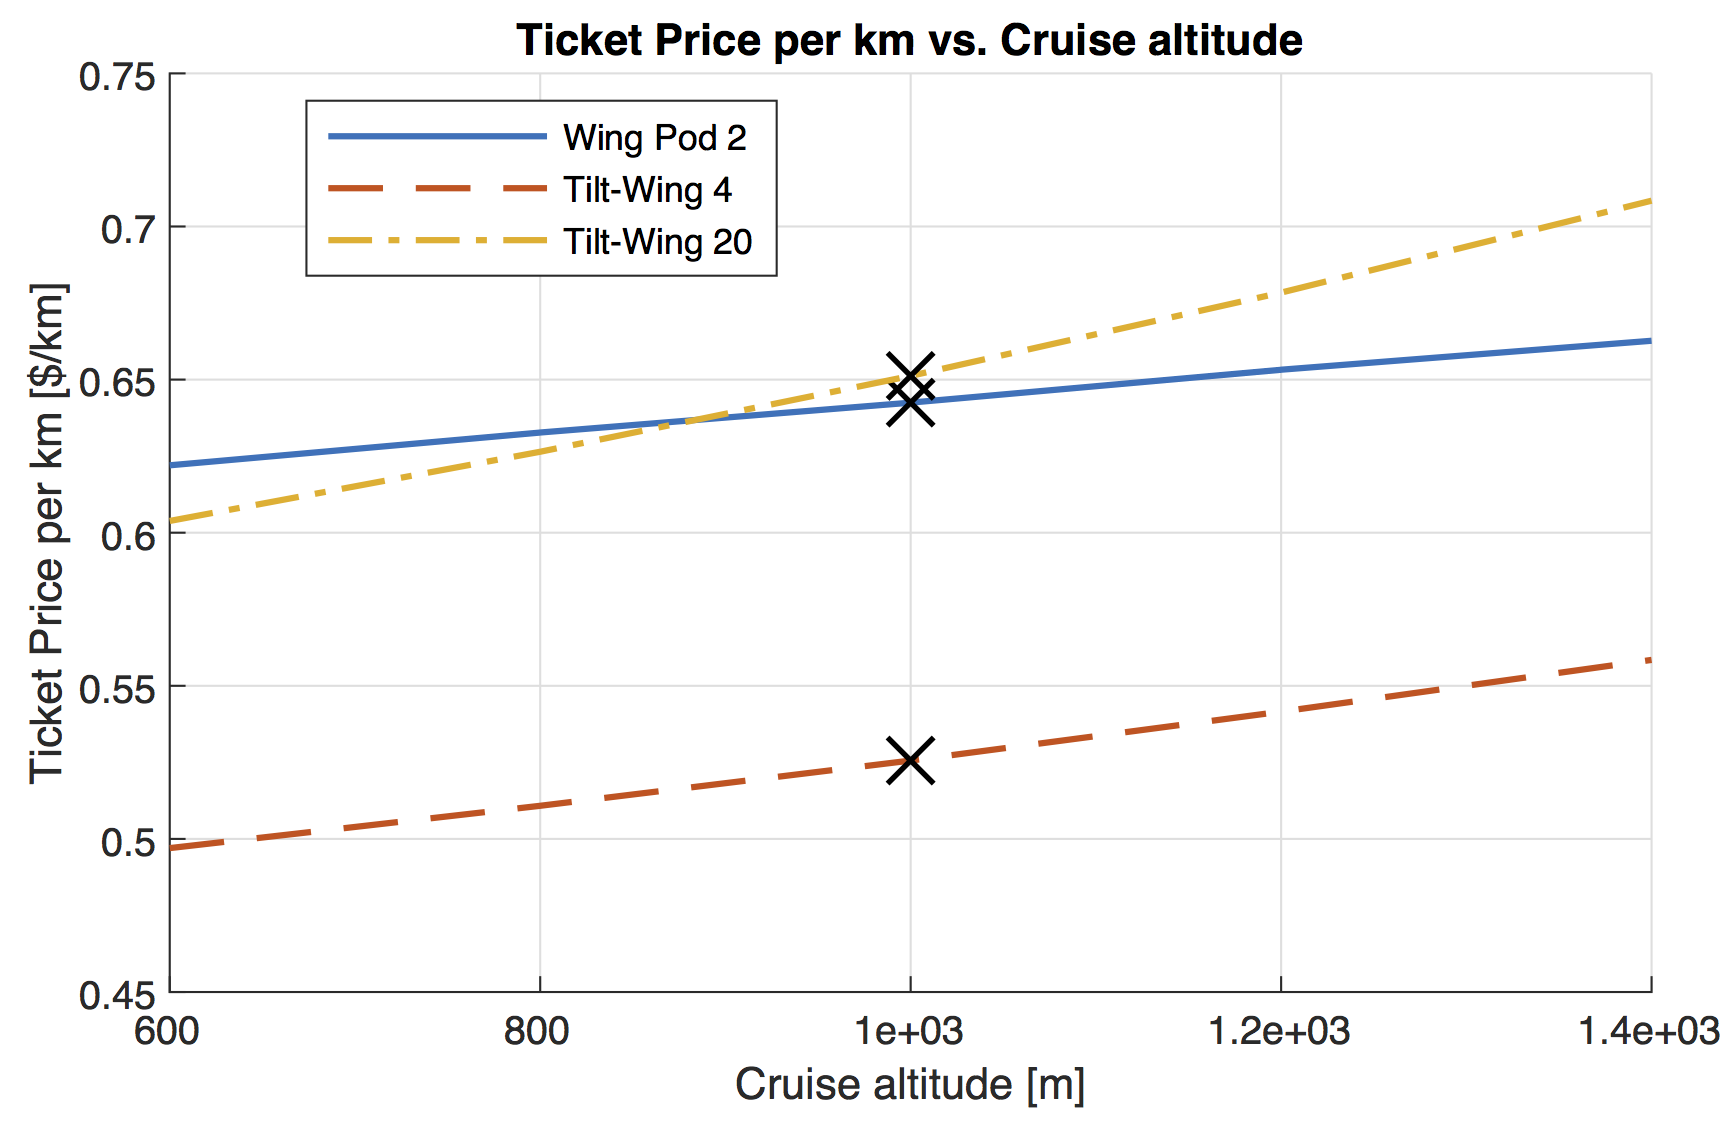
\includegraphics[width=\textwidth]{Figures/Alt_TPrice_perkmNOPAD.png}
    \captionsetup{justification=centering}
    \caption{Ticket price per km vs. Cruise Altitude}
    \label{fig:sens3} %x
\end{subfigure}
\begin{subfigure}[t]{0.33\textwidth}
    \centering
    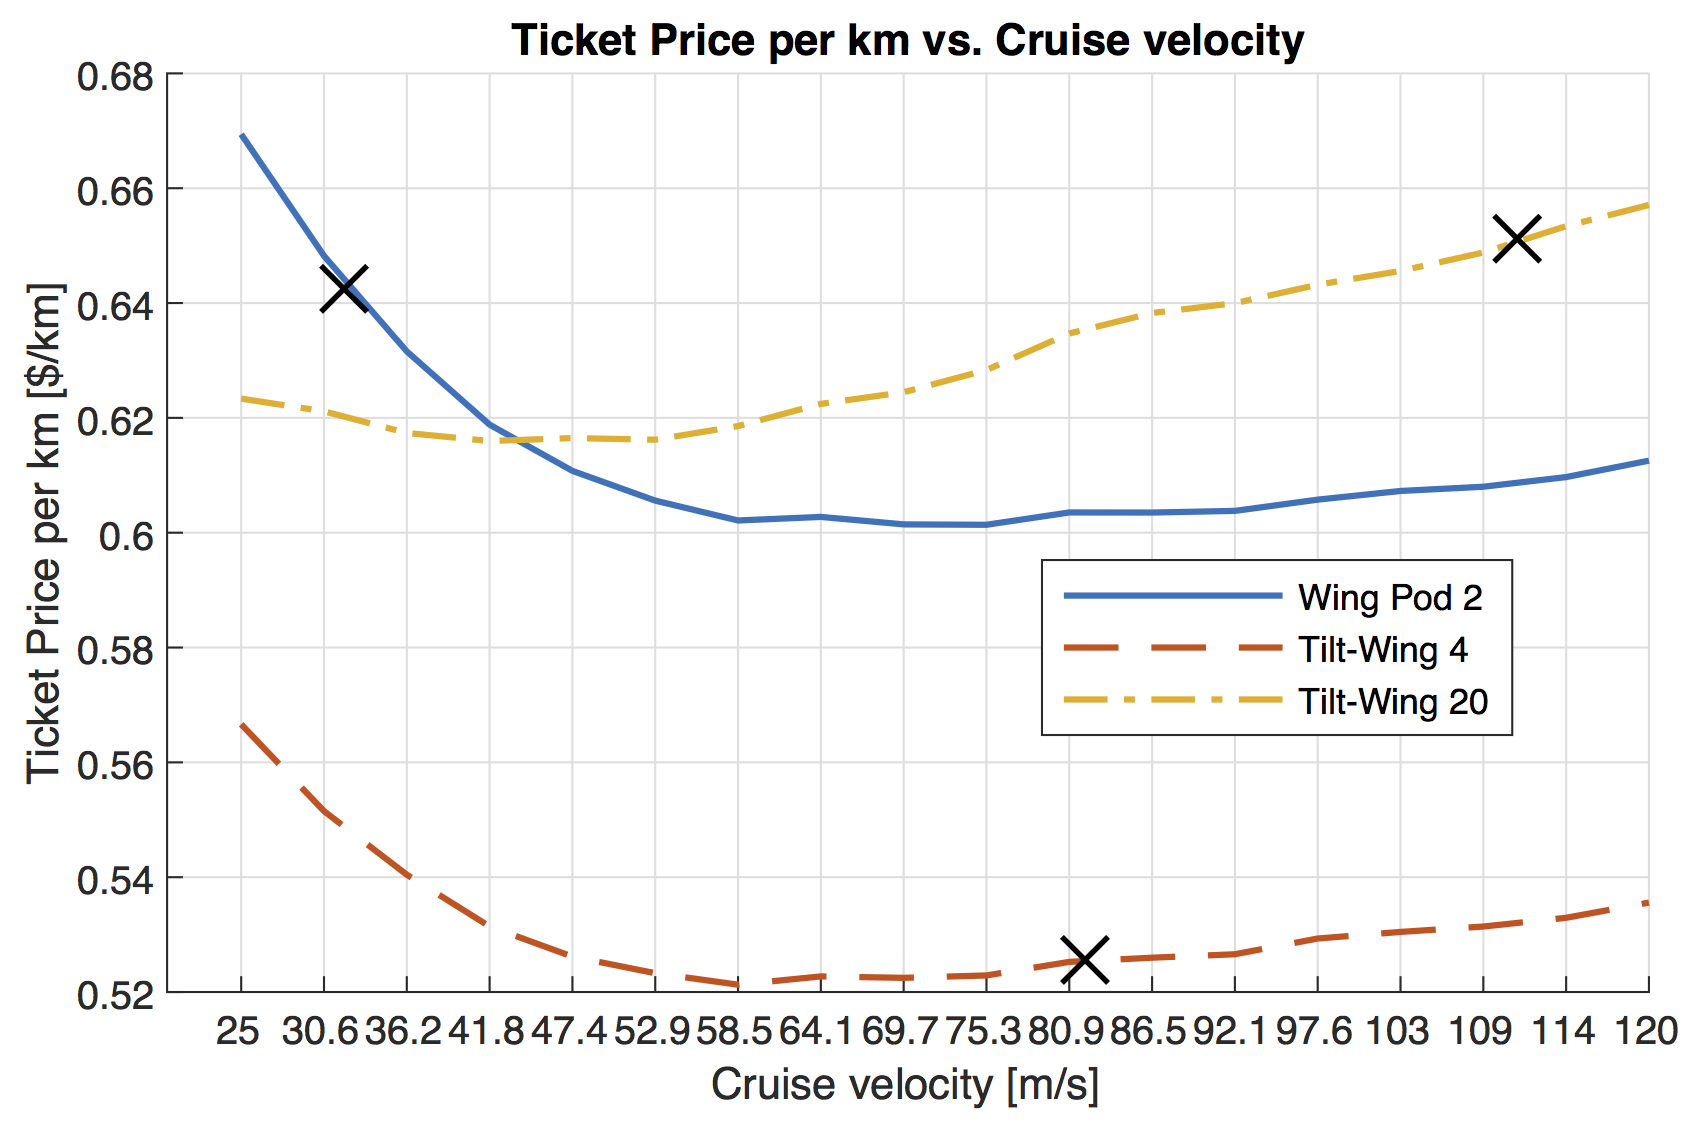
\includegraphics[width=\textwidth]{Figures/Cruise_TPrice_perkmNOPAD.png}
    \captionsetup{justification=centering}
    \caption{Ticket price per km vs. Cruise velocity}
    \label{fig:sens8}
\end{subfigure}
\begin{subfigure}[t]{0.33\textwidth}
    \centering
    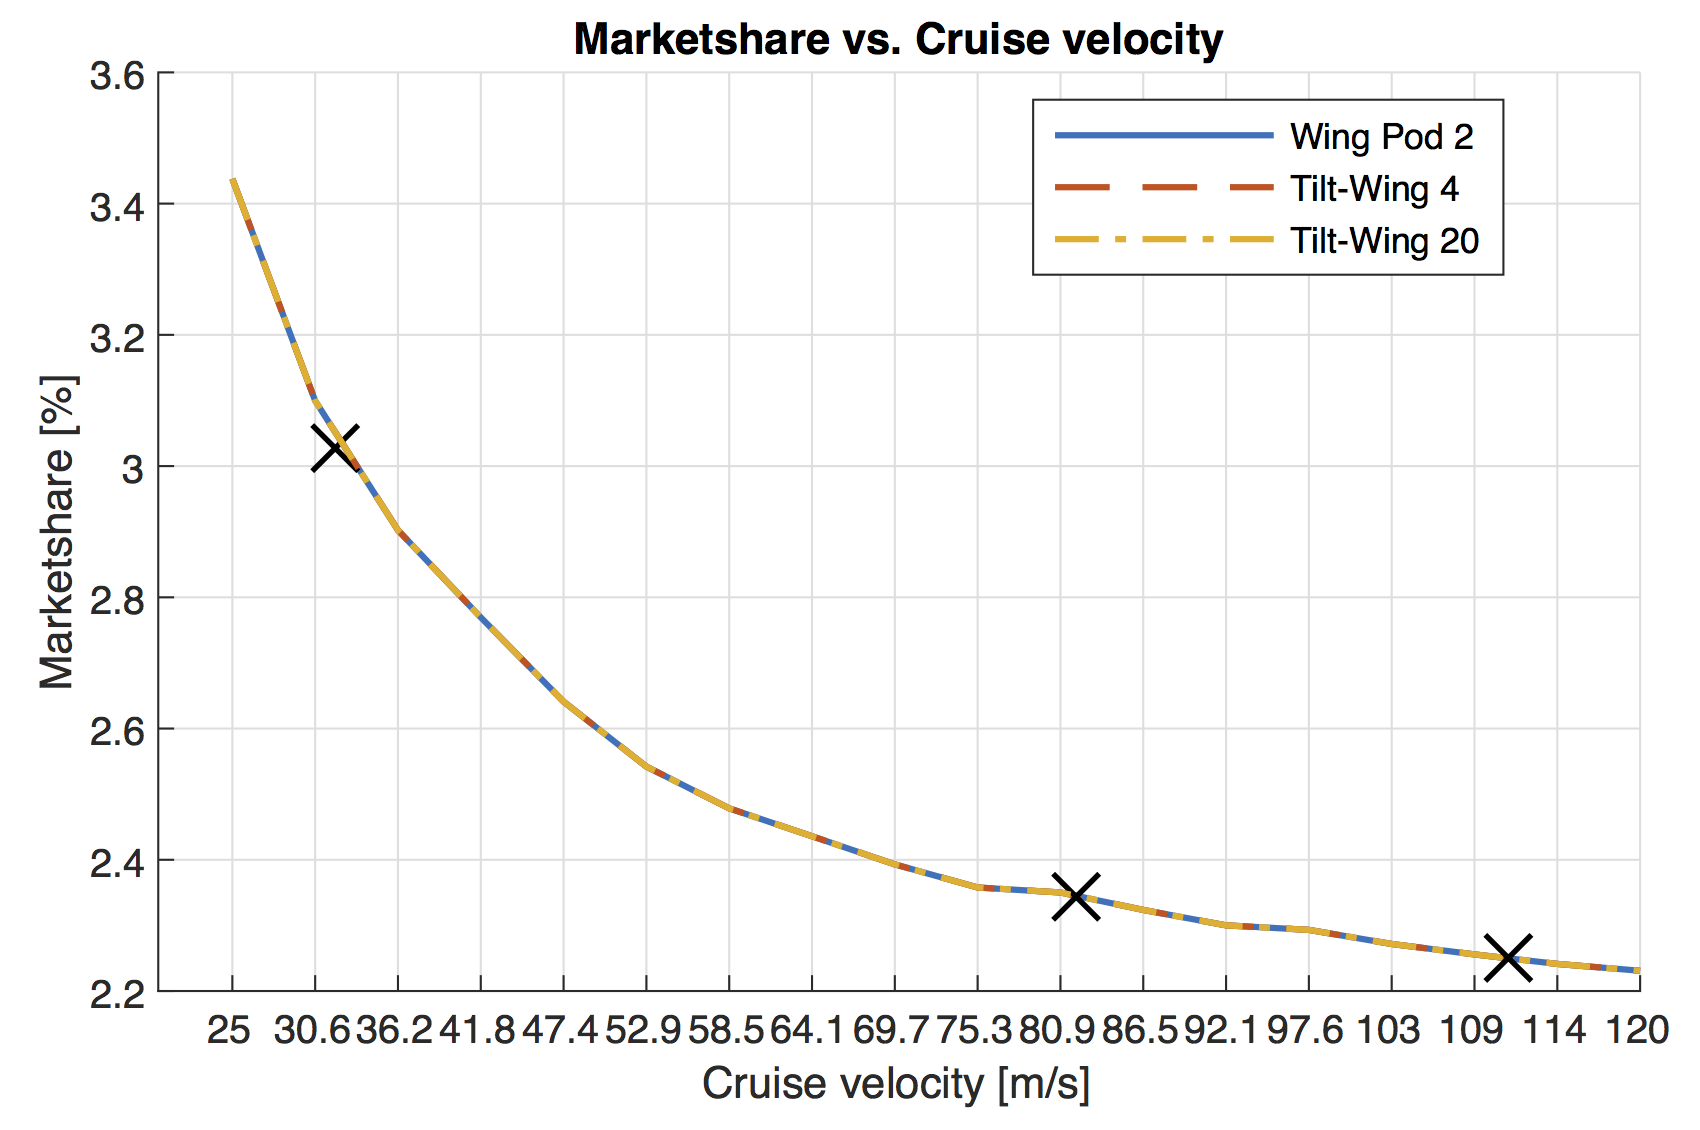
\includegraphics[width=\textwidth]{Figures/cruise_marketshare.png}
    \captionsetup{justification=centering}
    \caption{Market share vs. Cruise velocity}
    \label{fig:sens9}
\end{subfigure}
\captionsetup{justification=centering}
\end{figure}

\subsection{Cruise Velocity}
The cruise velocity is dependent on the vehicle design and has an important impact on the ticket price, due to its link with travel time. The ticket price change shown in \autoref{fig:sens8} is partly due to the change in market share (shown in \autoref{fig:sens9}). The shape of the plots are determined by the market share, but their translation is due to other sensitivities. Fortunately, there is a stand-out winner that may override those sensitivities.


\begin{figure}[10]{r}{0.35\textwidth}
    \centering
    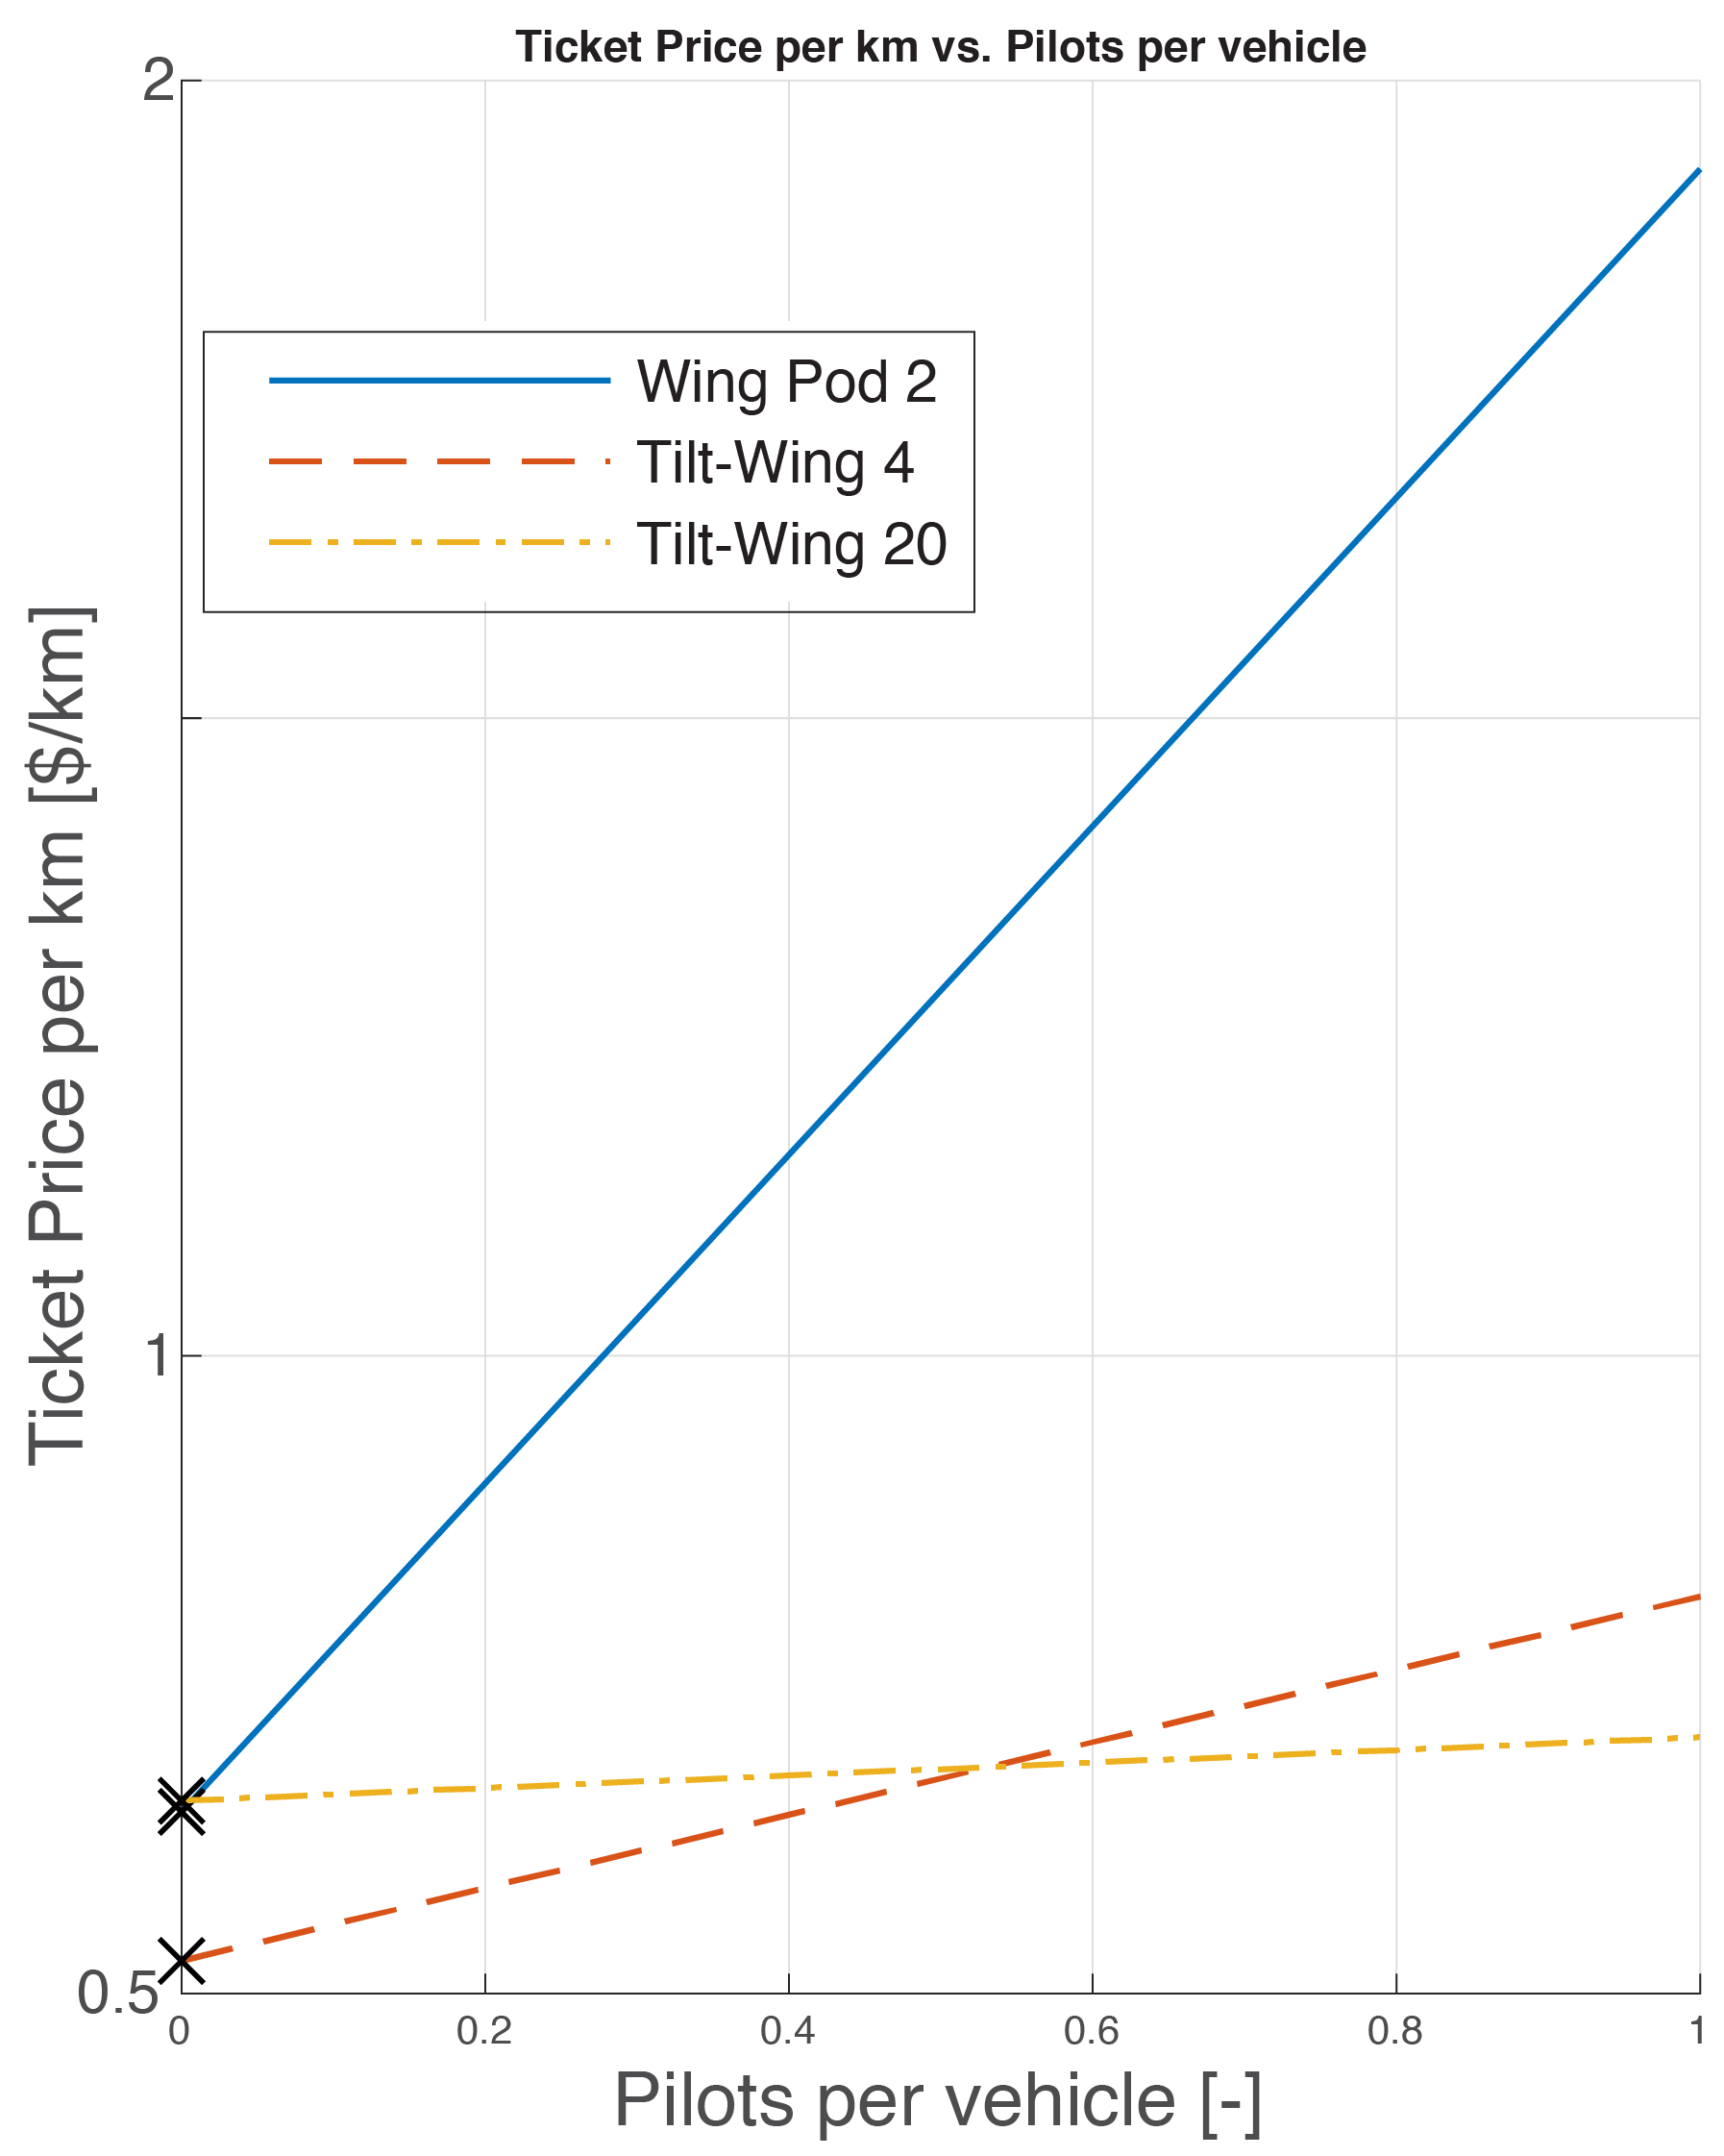
\includegraphics[width=0.35\textwidth]{Figures/autonomous_TPrice_perkm.png}
    \captionsetup{justification=centering}
    \caption{Ticket price increase due to including remote pilots, to assist autonomous vehicles.}
\label{fig:autocost}
\end{wrapfigure}


\subsection{Autonomous and Remotely Assisted Piloting}
Much of the trade-off has been done assuming that all the vehicles are completely autonomous. It is likely that remote piloting capabilities will be necessary for safety reasons. A pilot may need to intervene in certain situations. This also helps with a feeling of comfort for passengers. These pilots cost money, and will increase the operating cost per vehicle. By completing a sensitivity study based on the number of remote pilots, it can be shown at what point one concept may cost less than another. \autoref{fig:autocost} shows that the large vehicle benefits the most, and becomes cheaper (per km) to operate than the 4 passenger at 0.5 (1 pilot for every 2 vehicles). It seems more likely that less pilots will be required though.

\section{Trade-off Weight Sensitivity}

Once all of the scores were determined for the quantitative criteria, the qualitative scores also had to be calculated. The scores and weights were determined by the team using the AHP method described in \autoref{AHPMethod}. 

As part of the sensitivity analysis, a group of experts (including our client) were also asked to score the criteria using the AHP method. The resulting weights are given in \autoref{tab:toweights_expert} next to the weights given by the team. The final concept of the 4 passenger Tilt-wing concept remains the same.

While these two outcomes help assure the certainty of the trade-off, having even more scorings to compare would be more robust. To explore the sensitivity of the 11 weights, a simulation of different scoring was done. Using the scores of the three final concepts and the initial weights multiplied by random uniform variables, the outcomes of over 100000 different weight combinations was tallied. The 2 passenger concept only won in 7\% of the tallies. The 20 passenger concept did not win with any weighting combination. The weights that were high when the 2 passenger concept won were only the qualitative criteria, specifically passenger experience. 

Based on this analysis the 4 passenger concept is the strongest concept, unless there is a valid reason to more heavily value passenger experience.

% Please add the following required packages to your document preamble:
% \usepackage[table,xcdraw]{xcolor}
% If you use beamer only pass "xcolor=table" option, i.e. \documentclass[xcolor=table]{beamer}
\begin{table}[H]
\centering
\caption{Weights and Scores of Experts}
\label{tab:toweights_expert}
\begin{tabular}{lccccc}
\hline
\multicolumn{1}{c}{\textbf{Criteria}} & \textbf{\begin{tabular}[c]{@{}c@{}}Criteria Weights \\ (Team)\end{tabular}} & \textbf{\begin{tabular}[c]{@{}c@{}}Criteria Weights \\ (Expert)\end{tabular}} & \textbf{2 pax} & \textbf{4-6 pax} & \textbf{20 pax} \\ \hline
PREE & 0.278 & 0.360 & 5.00 & 5.00 & 3.00 \\
Battery mass & 0.078 & 0.108 & 4.00 & 5.00 & 3.00 \\
Safety & 0.185 & 0.135 & \cellcolor[HTML]{EFEFEF}2.67 & \cellcolor[HTML]{EFEFEF}3.00 & \cellcolor[HTML]{EFEFEF}4.00 \\
Passenger experience & 0.056 & 0.019 & \cellcolor[HTML]{EFEFEF}4.00 & \cellcolor[HTML]{EFEFEF}3.67 & \cellcolor[HTML]{EFEFEF}2.33 \\
Noise & 0.055 & 0.042 & 5.00 & 5.00 & 2.00 \\
Downwash & 0.017 & 0.020 & 5.00 & 5.00 & 4.00 \\
Development cost & 0.036 & 0.120 & \cellcolor[HTML]{EFEFEF}3.33 & \cellcolor[HTML]{EFEFEF}3.33 & \cellcolor[HTML]{EFEFEF}2.00 \\
Ticket price & 0.153 & 0.066 & 2.00 & 5.00 & 2.00 \\
ATM/UTM efforts & 0.081 & 0.041 & 1.40 & 2.70 & 2.90 \\
Weather conditions & 0.043 & 0.074 & \cellcolor[HTML]{EFEFEF}2.00 & \cellcolor[HTML]{EFEFEF}3.33 & \cellcolor[HTML]{EFEFEF}4.33 \\
Modification of regulations & 0.018 & 0.015 & \cellcolor[HTML]{EFEFEF}3.33 & \cellcolor[HTML]{EFEFEF}2.67 & \cellcolor[HTML]{EFEFEF}2.67 \\ \hline
\multicolumn{1}{c}{Sum of Weighted Scores of Experts} & \multicolumn{1}{l}{} &  & \cellcolor[HTML]{FFFC9E}\textbf{3.77} & \cellcolor[HTML]{67FD9A}\textbf{4.25} & \cellcolor[HTML]{FD6864}\textbf{3.00} \\ \hline
Sum of Weights Scores of Team & \multicolumn{1}{l}{} & \multicolumn{1}{l}{} & \cellcolor[HTML]{FFFC9E}\textbf{3.55} & \cellcolor[HTML]{67FD9A}\textbf{4.22} & \cellcolor[HTML]{FD6864}\textbf{2.65} \\ \hline
\end{tabular}
\end{table}


